\begin{figure}
	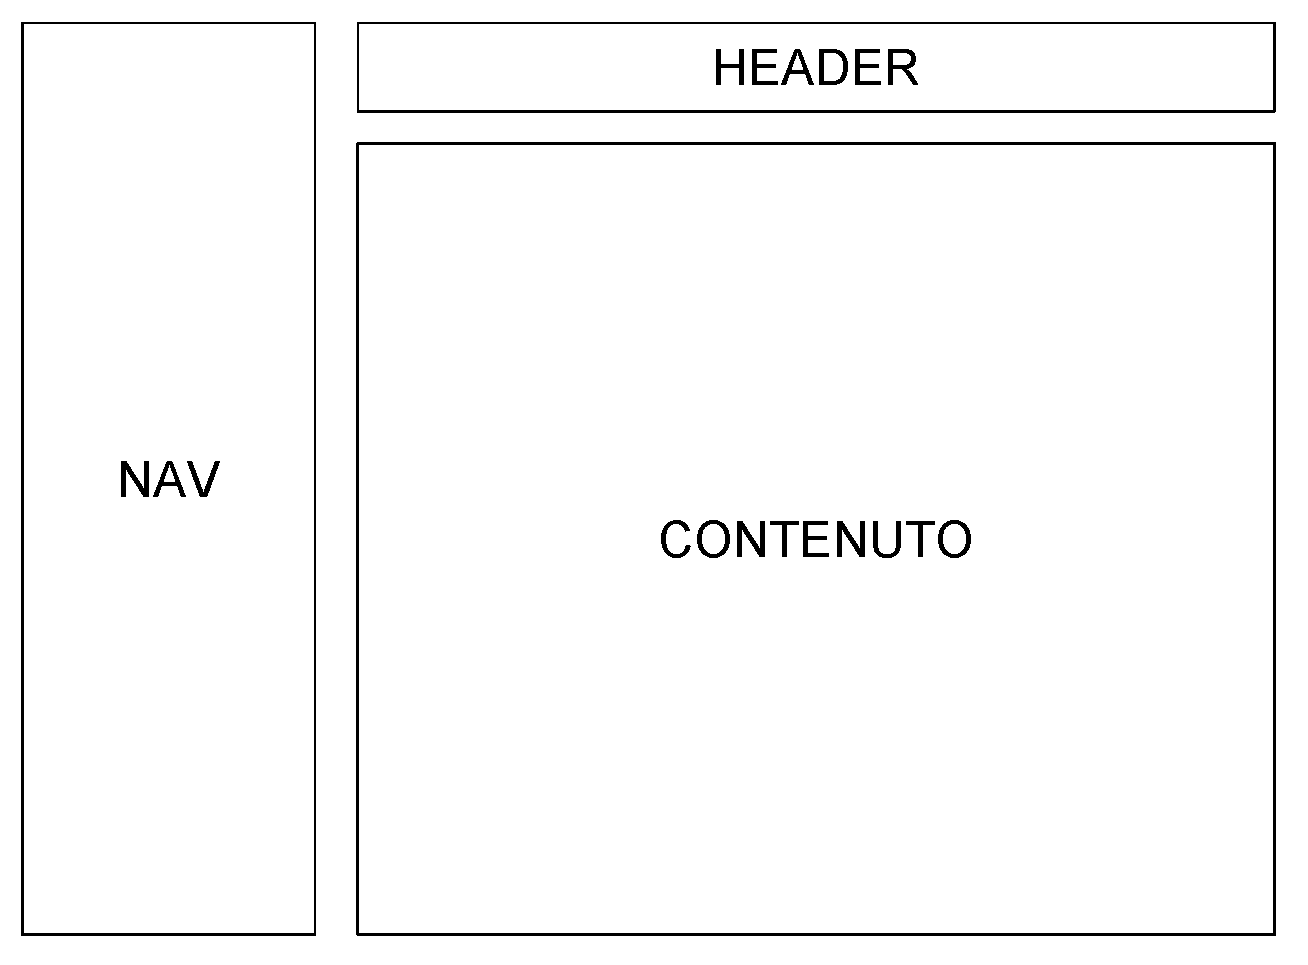
\includegraphics[width=1\linewidth]{sez/Progettazione/layout-base.pdf}
	\caption{Layout di una generica pagina del sito}
	\label{Fig:layoutBase}
\end{figure}

Per il sito è stato scelto un \textit{layout a tre pannelli}, come illustrato in \autoref{Fig:layoutBase}. Tale modello garantisce una superiore flessibilità e facilità di modifica in caso di aggiunta o rimozione di contenuti, e una maggiore adattabilità a taglie di schermo differenti. Ogni pagina del sito segue questo schema.